\chapter{Phương pháp đề xuất}
Như đã phân tích trong Chương 2, mô hình LayoutLMv3 \cite{huang2022layoutlmv3} tuy sở hữu biểu diễn đa phương thức mạnh mẽ nhưng vẫn thiếu các chỉ báo cấu trúc phân cấp tường minh ở đầu vào, thiếu cơ chế trao đổi ngữ cảnh trực tiếp ở cấp độ phân đoạn và chưa có ràng buộc giám sát ranh giới giữa các cặp token liên tiếp. Để giải quyết triệt để ba vấn đề này, khóa luận xây dựng mô hình mở rộng định hướng cấu trúc (\texttt{LayoutLMv3For}\allowbreak\texttt{Segment}\allowbreak\texttt{Token}\allowbreak\texttt{Classification}) bao gồm ba mô-đun cốt lõi hoạt động phối hợp: (1) \textbf{Mã hóa vị trí phân cấp HPE (Hierarchical Position Encoding)}, (2) \textbf{Mô-đun ngữ cảnh phân đoạn SCM (Segment Context Module)} tích hợp cổng dư ReZero và nhúng đánh dấu token đầu phân đoạn, và (3) \textbf{Hàm mất mát ranh giới nội dòng}. Ngoài ra, hệ thống còn hỗ trợ chiến lược tối ưu hóa tốc độ học phân biệt (\texttt{CustomTrainer}). Kiến trúc tổng thể của hệ thống đề xuất được minh họa trong Hình \ref{fig:proposed_architecture}.

\begin{figure}[htbp]
\centering
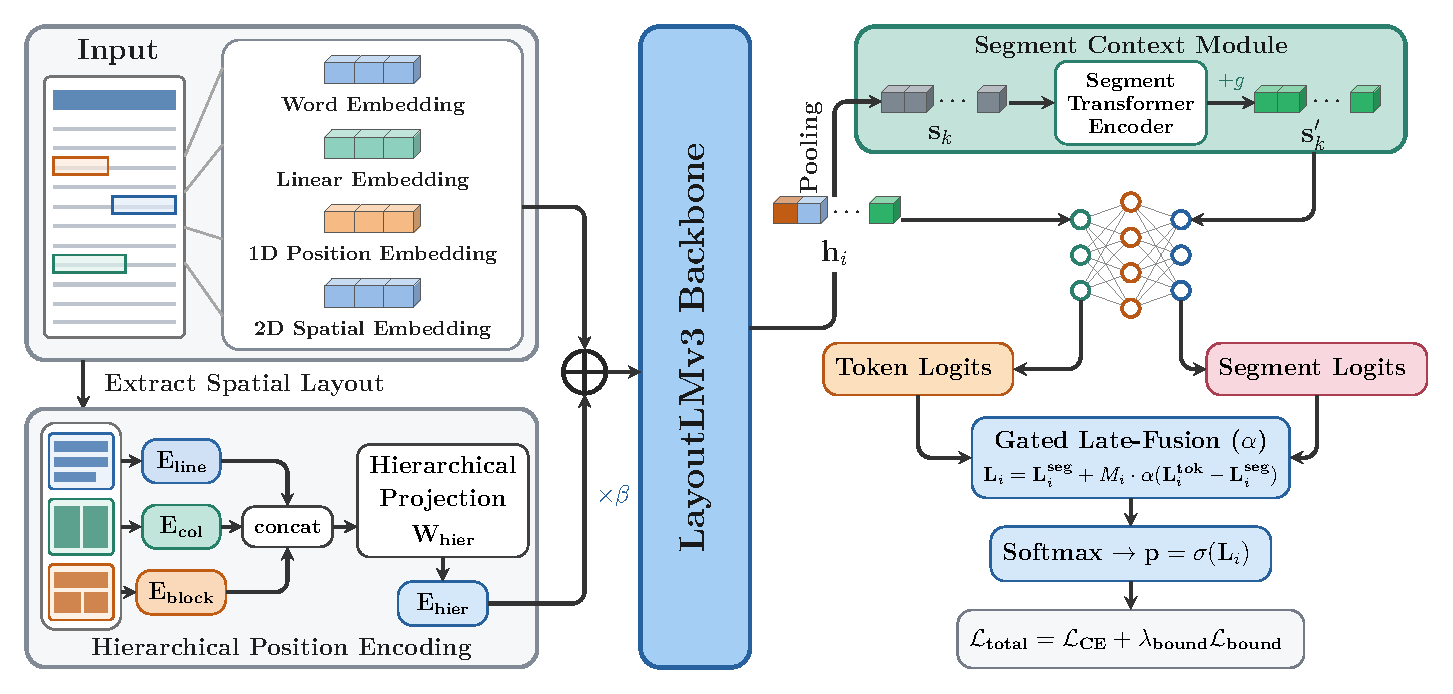
\includegraphics[width=\linewidth]{../figures/model_architecture_heads_style.pdf}
\caption{Kiến trúc tổng thể của khung mô hình LayoutLMv3 nhận thức cấu trúc cho bài toán Trích xuất thông tin chính KIE trên tài liệu giàu thị giác, tích hợp: (1) Mã hóa vị trí phân cấp HPE, (2) Bộ mã hóa xương sống LayoutLMv3 đa phương thức, (3) Mô-đun ngữ cảnh phân đoạn hai nhánh SCM kết hợp cổng dư ReZero, (4) Nhánh tắt bảo toàn độ mịn mức token, và (5) Bộ dung hợp trễ có cổng mặt nạ cấu trúc tối ưu đồng thời bởi hàm mất mát phân loại và hàm mất mát ranh giới nội dòng.}
\label{fig:proposed_architecture}
\end{figure}



\section{Mã hóa vị trí phân cấp HPE (Hierarchical Position Encoding)}
\subsection{Gom cụm hình học xác định chỉ số Dòng, Khối và Cột}
Trong giai đoạn tiền xử lý (\texttt{tokenize\_and\_}\allowbreak\texttt{align\_labels}), với mỗi từ gốc thứ $m \in \{0, 1, \dots, M-1\}$ có hộp giới hạn chuẩn hóa $\mathbf{b}_m = (x_0^{(m)}, y_0^{(m)}, x_1^{(m)}, y_1^{(m)}) \in [0, 1000]^4$, hệ thống tính tọa độ tâm ngang và tâm dọc của hộp giới hạn:
\begin{equation}
    x_c(m) = \frac{x_0^{(m)} + x_1^{(m)}}{2}, \qquad y_c(m) = \frac{y_0^{(m)} + y_1^{(m)}}{2}.
\end{equation}
Ba thuật toán gom cụm tuần tự dựa trên ngưỡng khoảng cách hình học được thực thi để trích xuất các chỉ số phân cấp:
\begin{enumerate}
    \item \textbf{Chỉ số dòng (\texttt{line\_ids}):} Khởi tạo $\text{id}_{\text{line}}(0) = 0$. Với mỗi từ $m \ge 1$, nếu khoảng cách tâm dọc so với từ liền trước vượt quá ngưỡng $\tau_{\text{line}}^y = 10$, chỉ số dòng tăng thêm 1:
    \begin{equation}
        \text{id}_{\text{line}}(m) = \text{id}_{\text{line}}(m-1) + \mathds{1}\!\left( \left| y_c(m) - y_c(m-1) \right| > \tau_{\text{line}}^y \right).
    \end{equation}
    \item \textbf{Chỉ số khối cục bộ (\texttt{block\_ids}):} Khởi tạo $\text{id}_{\text{block}}(0) = 0$. Hai từ liên tiếp được tách sang khối mới nếu độ lệch tâm ngang vượt quá $\tau_{\text{block}}^x = 50$ hoặc độ lệch tâm dọc vượt quá $\tau_{\text{block}}^y = 30$:
    \begin{equation}
    \begin{split}
        \text{id}_{\text{block}}(m) = \text{id}_{\text{block}}(m-1) + \mathds{1}\Big( &\left| x_c(m) - x_c(m-1) \right| > \tau_{\text{block}}^x \\
        &\lor\; \left| y_c(m) - y_c(m-1) \right| > \tau_{\text{block}}^y \Big).
    \end{split}
    \end{equation}
    \item \textbf{Chỉ số cột dọc (\texttt{column\_ids}):} Khởi tạo $\text{id}_{\text{col}}(0) = 0$. Khi độ lệch tâm ngang giữa hai từ liên tiếp vượt ngưỡng $\tau_{\text{col}}^x = 50$, chỉ số cột tăng thêm 1:
    \begin{equation}
        \text{id}_{\text{col}}(m) = \text{id}_{\text{col}}(m-1) + \mathds{1}\!\left( \left| x_c(m) - x_c(m-1) \right| > \tau_{\text{col}}^x \right).
    \end{equation}
\end{enumerate}

Khi một từ gốc $w_m$ được phân tách thành nhiều token con subword, toàn bộ các token con của từ đó kế thừa chung bộ ba chỉ số $\left(\text{id}_{\text{line}}(m), \text{id}_{\text{block}}(m), \text{id}_{\text{col}}(m)\right)$, trong khi các token đặc biệt (\texttt{<s>}, \texttt{</s>}, \texttt{<pad>}) và các mảnh ảnh thị giác được gán giá trị đệm $-1$.

\subsection{Phép chiếu nhúng phân cấp có trọng số giảm chấn cột}
Tại tầng nhúng \texttt{LayoutLMv3Embeddings}, ba bảng tra cứu nhúng học được được khởi tạo với kích thước chiều tọa độ $d_{\text{coord}}$ ($d_{\text{coord}} = 128$):
\begin{equation}
    \mathbf{E}_{\text{line}} \in \mathbb{R}^{N_{\text{line}} \times d_{\text{coord}}}, \quad
    \mathbf{E}_{\text{block}} \in \mathbb{R}^{N_{\text{block}} \times d_{\text{coord}}}, \quad
    \mathbf{E}_{\text{col}} \in \mathbb{R}^{N_{\text{col}} \times d_{\text{coord}}},
\end{equation}
trong đó $(N_{\text{line}}, N_{\text{block}}, N_{\text{col}})$ lần lượt là số lượng dòng, khối và cột tối đa (đặt là $(50, 20, 10)$ trên tập FUNSD và $(80, 15, 8)$ trên tập CORD). Để tránh lỗi vượt chỉ số bảng tra cứu, các chỉ số đầu vào được kẹp về miền hợp lệ $\tilde{\text{id}}_l(i) = \text{clamp}(\text{id}_{\text{line}}(i), 0, N_{\text{line}}-1)$ (tương tự cho $\tilde{\text{id}}_b(i)$ và $\tilde{\text{id}}_c(i)$).

Để giảm thiểu nhiễu phương sai từ phép gom cụm cột trên các bố cục phức tạp, véc-tơ nhúng cột được nhân với trọng số giảm chấn $\gamma_{\text{col}} = 0.3$ trước khi ghép nối với nhúng dòng và nhúng khối, sau đó đi qua lớp chiếu tuyến tính $\mathbf{W}_{\text{hier}} \in \mathbb{R}^{d_{\text{model}} \times (3 d_{\text{coord}})}$:
\begin{equation}
    \label{eq:hier_proj_impl}
    \mathbf{e}_i^{\text{hier}} = \mathbf{W}_{\text{hier}} \left[ \mathbf{E}_{\text{line}}\!\left(\tilde{\text{id}}_l(i)\right) \;\Vert\; \mathbf{E}_{\text{block}}\!\left(\tilde{\text{id}}_b(i)\right) \;\Vert\; \gamma_{\text{col}} \cdot \mathbf{E}_{\text{col}}\!\left(\tilde{\text{id}}_c(i)\right) \right] + \mathbf{b}_{\text{hier}}.
\end{equation}
Cuối cùng, biểu diễn vị trí phân cấp $\mathbf{e}_i^{\text{hier}}$ được cộng vào biểu diễn nhúng cơ sở $\mathbf{x}_i^{\text{text}}$ (Công thức \ref{eq:base_text_emb}) và đi qua lớp chuẩn hóa \texttt{LayerNorm} thứ hai để cân bằng phân phối kích hoạt trước khi tiến vào bộ mã hóa Transformer:
\begin{equation}
    \label{eq:total_emb_impl}
    \mathbf{x}_i^{\text{total}} = \text{Dropout}\!\left(\text{LayerNorm}\!\left(\mathbf{x}_i^{\text{text}} + \mathbf{e}_i^{\text{hier}}\right)\right).
\end{equation}

\section{Mô-đun ngữ cảnh phân đoạn SCM (Segment Context Module)}
\subsection{Khôi phục ranh giới phân đoạn và gộp trung bình}
Trong các tập dữ liệu chuẩn sử dụng bố cục mức phân đoạn (\texttt{--segment\_}\allowbreak\texttt{level\_}\allowbreak\texttt{layout 1}), các từ thuộc cùng một vùng/dòng OCR chia sẻ chính xác cùng một hộp giới hạn bao quanh. Dựa trên tính chất này, thuật toán tiền xử lý tái tạo chỉ số phân đoạn $\text{seg\_id}(i) \in \{0, 1, \dots, K-1\}$ theo thứ tự đọc bằng cách gán cùng mã phân đoạn $k$ cho dãy từ liên tiếp có hộp giới hạn trùng nhau ($\mathbf{b}_m = \mathbf{b}_{m-1}$), và gán $\text{seg\_id}(i) = -1$ cho token đặc biệt, token đệm hoặc mảnh ảnh.

Gọi $\mathbf{H}^{\text{out}} \in \mathbb{R}^{(L + 197) \times d_{\text{model}}}$ là đầu ra của lớp Transformer cuối cùng thuộc mạng xương sống LayoutLMv3. Mô hình tách riêng phần biểu diễn ẩn của chuỗi văn bản $\mathbf{H}^{\text{text}} = \mathbf{H}_{1:L}^{\text{out}} \in \mathbb{R}^{L \times d_{\text{model}}}$ và phần biểu diễn ẩn của chuỗi mảnh ảnh $\mathbf{H}^{\text{vis}} = \mathbf{H}_{L+1:L+197}^{\text{out}} \in \mathbb{R}^{197 \times d_{\text{model}}}$. Với mỗi phân đoạn hợp lệ $k \in \{0, 1, \dots, K-1\}$ chứa tập các vị trí token $S_k = \{i \in \{1, \dots, L\} \mid \text{seg\_id}(i) = k\}$, véc-tơ đại diện phân đoạn $\mathbf{s}_k \in \mathbb{R}^{d_{\text{model}}}$ được tính bằng phép gộp trung bình:
\begin{equation}
    \label{eq:seg_mean_pool_ch3}
    \mathbf{s}_k = \frac{1}{|S_k|} \sum_{i \in S_k} \mathbf{h}_i^{\text{text}}.
\end{equation}

\subsection{Trao đổi ngữ cảnh liên phân đoạn qua cổng dư ReZero và nhúng Token đầu}
Chuỗi gồm $K$ véc-tơ phân đoạn $\mathbf{S} = [\mathbf{s}_0, \mathbf{s}_1, \dots, \mathbf{s}_{K-1}] \in \mathbb{R}^{K \times d_{\text{model}}}$ được đưa qua một bộ mã hóa Transformer 1 lớp với $N_{\text{head}}^{\text{seg}} = 4$ đầu tự chú ý và số chiều tầng truyền thẳng $d_{\text{ffn}}^{\text{seg}} = 2 d_{\text{model}}$:
\begin{equation}
    \label{eq:seg_transformer_ch3}
    \mathbf{C} = [\mathbf{c}_0, \mathbf{c}_1, \dots, \mathbf{c}_{K-1}] = \text{SegmentTransformerEncoder}(\mathbf{S}).
\end{equation}
Do số lượng phân đoạn $K$ trong một tài liệu thường rất nhỏ ($K \approx 20\text{--}60 \ll L \le 512$), độ phức tạp tự chú ý của bước này chỉ là $\mathcal{O}(K^2)$, hầu như không làm tăng chi phí tính toán. Tiếp theo, cổng dư ReZero \cite{bachlechner2021rezero} với tham số vô hướng học được $g \in \mathbb{R}$ (khởi tạo $g = 0$) điều tiết lượng thông tin ngữ cảnh liên phân đoạn được hòa trộn vào véc-tơ gốc:
\begin{equation}
    \label{eq:rezero_blend_ch3}
    \mathbf{s}'_k = \mathbf{s}_k + g \cdot (\mathbf{c}_k - \mathbf{s}_k).
\end{equation}
Tại bước huấn luyện $t = 0$, do $g = 0$ nên $\mathbf{s}'_k = \mathbf{s}_k$, đảm bảo các trọng số ngẫu nhiên của \texttt{SegmentTransformerEncoder} không gây nhiễu loạn gradient truyền ngược về mạng xương sống đã tiền huấn luyện.

Sau khi phát tán $\mathbf{s}'_k$ về lại từng token $i \in S_k$, mọi token trong cùng phân đoạn $S_k$ đều mang cùng một véc-tơ $\mathbf{s}'_k$. Để bộ phân loại ở tầng cuối vẫn phân biệt được token mở đầu phân đoạn (cần dự đoán nhãn $\text{B-}c$) với các token đứng sau trong cùng phân đoạn (cần dự đoán nhãn $\text{I-}c$), khóa luận bổ sung một bảng nhúng nhị phân học được $\mathbf{E}_{\text{first}} \in \mathbb{R}^{2 \times d_{\text{model}}}$ (khởi tạo theo phân phối chuẩn $\mathcal{N}(0, 0.02^2)$). Cờ chỉ thị vị trí đầu phân đoạn $f_i \in \{0, 1\}$ cho token thứ $i$ được xác định tự động:
\begin{equation}
    \label{eq:is_first_flag}
    f_i = \mathds{1}\!\left(\text{seg\_id}(i) \ge 0 \;\land\; \text{seg\_id}(i) \neq \text{seg\_id}(i-1)\right),
\end{equation}
và biểu diễn ẩn văn bản sau làm giàu phân đoạn $\tilde{\mathbf{h}}_i^{\text{text}}$ được tính bởi:
\begin{equation}
    \label{eq:broadcast_with_first}
    \tilde{\mathbf{h}}_i^{\text{text}} = \begin{cases}
        \mathbf{s}'_{\text{seg\_id}(i)} + \mathbf{E}_{\text{first}}(f_i), & \text{nếu } \text{seg\_id}(i) \ge 0, \\
        \mathbf{h}_i^{\text{text}} + \mathbf{E}_{\text{first}}(0), & \text{nếu } \text{seg\_id}(i) = -1.
    \end{cases}
\end{equation}

\section{Hàm mất mát ranh giới nội dòng/thực thể}
\subsection{Thuật toán gán mã định danh thực thể liên tục (\texttt{compute\_entity\_ids})}
Nhằm khắc phục việc thiếu giám sát trực tiếp tại điểm chuyển tiếp giữa hai thực thể liền kề, khóa luận thiết kế hàm mất mát ranh giới dựa trên chuỗi mã định danh thực thể liên tục $\text{ent}_i \in \{-1, 0, 1, \dots\}$. Khác với các quy tắc dựa trên tính chẵn/lẻ của mã nhãn vốn phụ thuộc vào thứ tự bảng chữ cái của tập nhãn, hàm \texttt{compute\_entity\_ids} trích xuất định danh thực thể tổng quát trực tiếp từ tiền tố $\text{B-}/\text{I-}$ và tên loại thực thể $c$ của chuỗi nhãn chuẩn $y_1, \dots, y_L$:
\begin{itemize}
    \item Nếu token thứ $i$ có nhãn bị bỏ qua ($y_i = -100$) hoặc nhãn nền ($y_i = \text{``O''}$), gán $\text{ent}_i = -1$ và đặt lại trạng thái loại thực thể trước đó $\text{prev\_type} \gets \text{None}$.
    \item Nếu token thứ $i$ mang nhãn thực thể có dạng $\text{``prefix-etype''}$ (với $\text{prefix} \in \{\text{B}, \text{I}\}$): mỗi khi gặp tiền tố $\text{prefix} = \text{``B''}$ hoặc khi loại thực thể hiện tại khác với loại thực thể liền trước ($\text{etype} \neq \text{prev\_type}$), bộ đếm thực thể tăng thêm 1 ($\text{current\_id} \gets \text{current\_id} + 1$) và gán $\text{ent}_i = \text{current\_id}$. Các token tiếp nối hợp lệ ($\text{prefix} = \text{``I''}$ và $\text{etype} = \text{prev\_type}$) giữ nguyên mã $\text{current\_id}$ của thực thể hiện tại.
\end{itemize}
Nhờ cơ chế này, hai token thực thể liên tiếp $(i, i+1)$ có $\text{ent}_i = \text{ent}_{i+1}$ khi và chỉ khi chúng thuộc cùng một thực thể thực tế duy nhất, và có $\text{ent}_i \neq \text{ent}_{i+1}$ khi có một ranh giới phân tách thực thể giữa chúng.

\subsection{Mạng phân loại ranh giới cặp Token và hàm mất mát nhị phân}
Lưu ý rằng sau bước gộp phân đoạn (Công thức \ref{eq:broadcast_with_first}), các token trong cùng một phân đoạn đã chia sẻ chung véc-tơ $\mathbf{s}'_k$. Do đó, để rèn luyện khả năng phân định ranh giới thực thể trực tiếp cho mạng xương sống LayoutLMv3, nhánh phân loại ranh giới hoạt động trên chuỗi biểu diễn ẩn văn bản \textbf{trước khi gộp phân đoạn} $\mathbf{h}_1^{\text{text}}, \dots, \mathbf{h}_L^{\text{text}}$.

Với mỗi cặp token liên tiếp $(i, i+1)$ ($1 \le i \le L-1$), hai véc-tơ ẩn được ghép nối thành $\mathbf{h}_{\text{pair}, i} = [\mathbf{h}_i^{\text{text}} \;\Vert\; \mathbf{h}_{i+1}^{\text{text}}] \in \mathbb{R}^{2 d_{\text{model}}}$ và đưa qua mạng MLP hai lớp (\texttt{boundary\_classifier}) để dự đoán điểm số logit ranh giới $z_i^{\text{bound}} \in \mathbb{R}$:
\begin{equation}
    \label{eq:boundary_mlp}
    z_i^{\text{bound}} = \mathbf{w}_2^\top \,\text{ReLU}\!\left( \mathbf{W}_1 \left[\mathbf{h}_i^{\text{text}} \;\Vert\; \mathbf{h}_{i+1}^{\text{text}}\right] + \mathbf{b}_1 \right) + b_2,
\end{equation}
với $\mathbf{W}_1 \in \mathbb{R}^{d_{\text{model}} \times 2 d_{\text{model}}}$ và $\mathbf{w}_2 \in \mathbb{R}^{d_{\text{model}}}$. Tập hợp các cặp chỉ số hợp lệ $\mathcal{V}_{\text{bound}}$ bao gồm các cặp token thực thể liên tiếp không bị che mặt nạ chú ý ($m_i = 1 \land m_{i+1} = 1$) và đều thuộc về các thực thể có tên ($\text{ent}_i \ge 0 \land \text{ent}_{i+1} \ge 0$):
\begin{equation}
    \mathcal{V}_{\text{bound}} = \left\{ i \in \{1, \dots, L-1\} \;\middle|\; \text{ent}_i \ge 0 \;\land\; \text{ent}_{i+1} \ge 0 \;\land\; m_i = 1 \;\land\; m_{i+1} = 1 \right\}.
\end{equation}
Nhãn ranh giới chuẩn cho cặp thứ $i \in \mathcal{V}_{\text{bound}}$ được định nghĩa là $y_i^{\text{bound}} = \mathds{1}(\text{ent}_i \neq \text{ent}_{i+1}) \in \{0, 1\}$. Hàm mất mát ranh giới nội dòng $\mathcal{L}_{\text{bound}}$ là mất mát Entropy chéo nhị phân:
\begin{equation}
    \label{eq:boundary_loss}
    \mathcal{L}_{\text{bound}} = -\frac{1}{|\mathcal{V}_{\text{bound}}|} \sum_{i \in \mathcal{V}_{\text{bound}}} \left[ y_i^{\text{bound}} \log \sigma\!\left(z_i^{\text{bound}}\right) + \left(1 - y_i^{\text{bound}}\right) \log \left(1 - \sigma\!\left(z_i^{\text{bound}}\right)\right) \right].
\end{equation}

Một chi tiết kỹ thuật quan trọng trong mã nguồn của khóa luận là hệ số trọng số $\lambda_{\text{bound}} = 0.1$ được lưu trữ dưới dạng \textbf{hằng số thực cố định} thay vì một tham số học được (\texttt{nn.Parameter}). Nếu $\lambda_{\text{bound}}$ được phép cập nhật tự do theo gradient của tổng hàm mất mát $\mathcal{L}_{\text{total}} = \mathcal{L}_{\text{CE}} + \lambda_{\text{bound}} \mathcal{L}_{\text{bound}}$, thuật toán hạ gradient sẽ lập tức đẩy $\lambda_{\text{bound}}$ về giá trị âm ($\lambda_{\text{bound}} \to -\infty$) để làm giảm giá trị hàm mục tiêu một cách giả tạo, qua đó đảo ngược hoàn toàn ý nghĩa của $\mathcal{L}_{\text{bound}}$.

\section{Quy trình huấn luyện tổng thể và tối ưu hóa tốc độ học phân biệt}
Tổng hợp các thành phần trên, toàn bộ quy trình lan truyền tiến và cập nhật tham số của mô hình đề xuất được trình bày chi tiết trong Thuật toán \ref{alg:proposed_training}.

\SetKwInput{KwInput}{Đầu vào}
\SetKwInput{KwOutput}{Đầu ra}
\SetKwInput{KwInit}{Khởi tạo}
\begin{algorithm}[htbp]
\small
\SetAlgoLined
\DontPrintSemicolon
\KwIn{Lô tài liệu đã mã hóa $\mathcal{B} = \{(\mathbf{w}, \mathbf{B}_{\text{box}}, \mathbf{s}, \mathbf{I}, \mathbf{y})\}$; hệ số $\lambda_{\text{bound}} = 0.2$.}
\KwOut{Logit phân loại token $\mathbf{Z} \in \mathbb{R}^{B \times L \times |\mathcal{Y}|}$ và hàm mất mát kết hợp $\mathcal{L}_{\text{total}}$.}

\BlankLine
\textbf{Bước 1: Mã hóa vị trí 2D phân cấp (HPE)}\;
\ForEach{token $i \in \{1, \dots, L\}$}{
    Nhúng tọa độ ngang $\mathbf{e}_{\text{horiz}}(\mathbf{b}_i)$ và tọa độ dọc $\mathbf{e}_{\text{vert}}(\mathbf{b}_i)$\;
    Chiếu phân cấp: $\mathbf{e}_{\text{HPE}}^{\text{pos2D}}(\mathbf{b}_i) \leftarrow \text{GELU}(\text{LN}(\mathbf{W}_{\text{HPE}}[\mathbf{e}_{\text{horiz}} \| \mathbf{e}_{\text{vert}}] + \mathbf{b}_{\text{HPE}}))$\;
    Tạo đầu vào chữ: $\mathbf{e}_i^{\text{text}} \leftarrow \text{LN}(\mathbf{e}^{\text{word}}(w_i) + \mathbf{e}^{\text{pos1D}}(i) + \mathbf{e}^{\text{type}}(0) + \mathbf{e}_{\text{HPE}}^{\text{pos2D}}(\mathbf{b}_i))$\;
}

\BlankLine
\textbf{Bước 2: Mã hóa đa phương thức bằng mạng xương sống Transformer}\;
Trích xuất mảnh ảnh $\mathbf{E}^{\text{image}} \in \mathbb{R}^{B \times (M+1) \times d}$ từ ảnh tài liệu $\mathbf{I}$\;
Mã hóa chuỗi đa phương thức: $\mathbf{H}_{\text{enc}} \leftarrow \text{TransformerEncoder}([\mathbf{E}^{\text{text}} \| \mathbf{E}^{\text{image}}])$\;
Lấy trạng thái ẩn token chữ: $\mathbf{H} = (\mathbf{h}_1, \dots, \mathbf{h}_L) \leftarrow \mathbf{H}_{\text{enc}}[:, :L, :]$\;

\BlankLine
\textbf{Bước 3: Tương tác ngữ cảnh phân đoạn (SCM) với cổng ReZero}\;
\ForEach{chỉ số phân đoạn $k \in \{0, \dots, S-1\}$}{
    Gộp trung bình token trong phân đoạn: $\mathbf{u}_k \leftarrow \frac{1}{\max(|\mathcal{I}_k|, 1)} \sum_{i \in \mathcal{I}_k} \mathbf{h}_i$\;
}
Cập nhật ngữ cảnh phân đoạn: $\hat{\mathbf{U}} \leftarrow \text{LN}_{\text{seg}}(\mathbf{U} + \text{Dropout}(\mathbf{W}_{\text{seg}}^O \text{MHSA}_{\text{seg}}(\mathbf{U})))$\;
\ForEach{token $i \in \{1, \dots, L\}$}{
    Chỉ số đầu đoạn $f_i \leftarrow \mathds{1}[s_i \ge 0 \wedge (i = 1 \vee s_i \neq s_{i-1})]$\;
    Dung hợp phân đoạn: $\mathbf{h}_i^{\text{final}} \leftarrow \mathbf{h}_i + \alpha \cdot \mathds{1}[s_i \ge 0] \cdot (\hat{\mathbf{u}}_{s_i} + \mathbf{e}_{\text{first}}(f_i))$\;
}

\BlankLine
\textbf{Bước 4: Logit phân loại \& Ràng buộc ranh giới nội dòng}\;
Tính logit $\mathbf{Z} \leftarrow \text{Classifier}(\text{Dropout}(\mathbf{H}^{\text{final}})) \in \mathbb{R}^{B \times L \times |\mathcal{Y}|}$\;
Tính mất mát Cross-Entropy $\mathcal{L}_{\text{CE}}(\mathbf{Z}, \mathbf{y})$ trên các token hợp lệ\;
Xác định cặp liền kề nội dòng: $\mathcal{P}_{\text{intra}} = \{(i, i+1) \mid s_i = s_{i+1} \ge 0, \, \phi(y_i) = \phi(y_{i+1})\}$\;
Tính mất mát cosin ranh giới: $\mathcal{L}_{\text{bound}} \leftarrow \frac{1}{|\mathcal{P}_{\text{intra}}|} \sum_{(i,i+1)} (1 - \cos(\mathbf{h}_i^{\text{final}}, \mathbf{h}_{i+1}^{\text{final}}))$\;
\Return{$\mathbf{Z}$ và $\mathcal{L}_{\text{total}} \leftarrow \mathcal{L}_{\text{CE}} + \lambda_{\text{bound}}\mathcal{L}_{\text{bound}}$}\;
\caption{Quy trình lan truyền tiến và huấn luyện kết hợp Structure-Aware LayoutLMv3}
\label{alg:proposed_training}
\end{algorithm}

Để đảm bảo các mô-đun khởi tạo ngẫu nhiên (\texttt{segment\_}\allowbreak\texttt{context}, \texttt{segment\_}\allowbreak\texttt{context\_}\allowbreak\texttt{gate}, \texttt{is\_first\_}\allowbreak\texttt{token\_}\allowbreak\texttt{embedding}, \texttt{boundary\_}\allowbreak\texttt{classifier} và \texttt{classifier}) hội tụ nhanh trong vòng $1000$ bước huấn luyện mà không làm phá vỡ tri thức tiền huấn luyện của mạng xương sống, bộ huấn luyện tùy chỉnh \texttt{CustomTrainer} chia toàn bộ tham số mô hình thành hai nhóm tốc độ học riêng biệt trong bộ tối ưu hóa AdamW:
\begin{itemize}
    \item \textbf{Nhóm tham số xương sống ($\theta_{\text{base}}$, gồm toàn bộ các tham số có tiền tố \texttt{"layoutlmv3"}):} Sử dụng tốc độ học nhỏ $\eta_{\text{base}}$ truyền từ cấu hình ($\eta_{\text{base}} = 1\times 10^{-5}$ trên FUNSD và $\eta_{\text{base}} = 5\times 10^{-5}$ trên CORD).
    \item \textbf{Nhóm tham số mô-đun mới ($\theta_{\text{new}}$, gồm SCM, cổng ReZero $g$, nhúng đầu phân đoạn, bộ phân loại ranh giới và đầu phân loại nhãn):} Sử dụng tốc độ học lớn hơn $\eta_{\text{new}} = 5\times 10^{-4}$ để tăng tốc độ thích ứng cấu trúc.
\end{itemize}

